
\section{Raspberry Pi}
\label{sec:Raspberry-Pi}

Após constatado que o ESP8266 não oferece modo promíscuo, como visto na \autoref{subsec:testes-esp}, foi testado e
desenvolvido software para transformar o Raspberry Pi em uma plataforma para
hospedar o sensor. Sua principal diferença é o sistema operacional linux
(inexistente no ESP8266) que favorece esta plataforma, porém seu alto custo a
desfavorece. Em média, no exterior, o RPI3 é vendido por USD \$ 35,00
\cite{RPI2016} e, no Brasil, entre R\$ 270 em Março de 2016 e R\$ 190 em Janeiro
de 2017 \cite{rpi3-mercadolivre}.

As vantagens de ter um computador moderno completo sobrepõem seu custo em muitas
vezes, dentre as quais destaca-se o poder computacional e a interface "amigável"
com usuário devido ao
sistema operacional oferecendo maior nível de abstração (bastando apenas alguns
comandos para acessá-los e realizar tarefas complexas).
Além deste recurso a nível de sistema, a comunidade e o número de projetos DIY
é muito maior que a do ESP8266, devido a sua simplicidade em
conectar-se a um monitor e construir protótipos e aplicações.

O RPI3 é um computador \emph{single-board}  (única
placa) que tem o tamanho próximo ao de um cartão de crédito. Como visto na \autoref{fig-rpi-3}, foi desenvolvido
pela Raspberry Pi Foundation para promover o ensino da computação nas
escolas. Este computador possui:


\begin{alineas}
	\item 1 GB RAM;

	\item Processador Gráfico VideoCore IV 3D;

	\item ARM CPU de 1.2 GHz quad-core 64-bit;

	\item 4 portas USB;

	\item 40 pinos GPIOs;

	\item Porta HDMI;

	\item Porta Megabit Ethernet;

	\item Saída de aúdio e vídeo 3.5 mm;

	\item Interface para câmera (CSI) e monitor (DSI);

	\item Leitor para cartão micro SD;

	\item \emph{Wi-Fi LAN} embutida 802.11n;

	\item Bluetooth 4.1 e \emph{Bluetooth Low Energy} (BLE).

\end{alineas}

\begin{figure}[htb]
	\caption{\label{fig-rpi-3}Raspberry Pi 3 }
	\begin{center}
		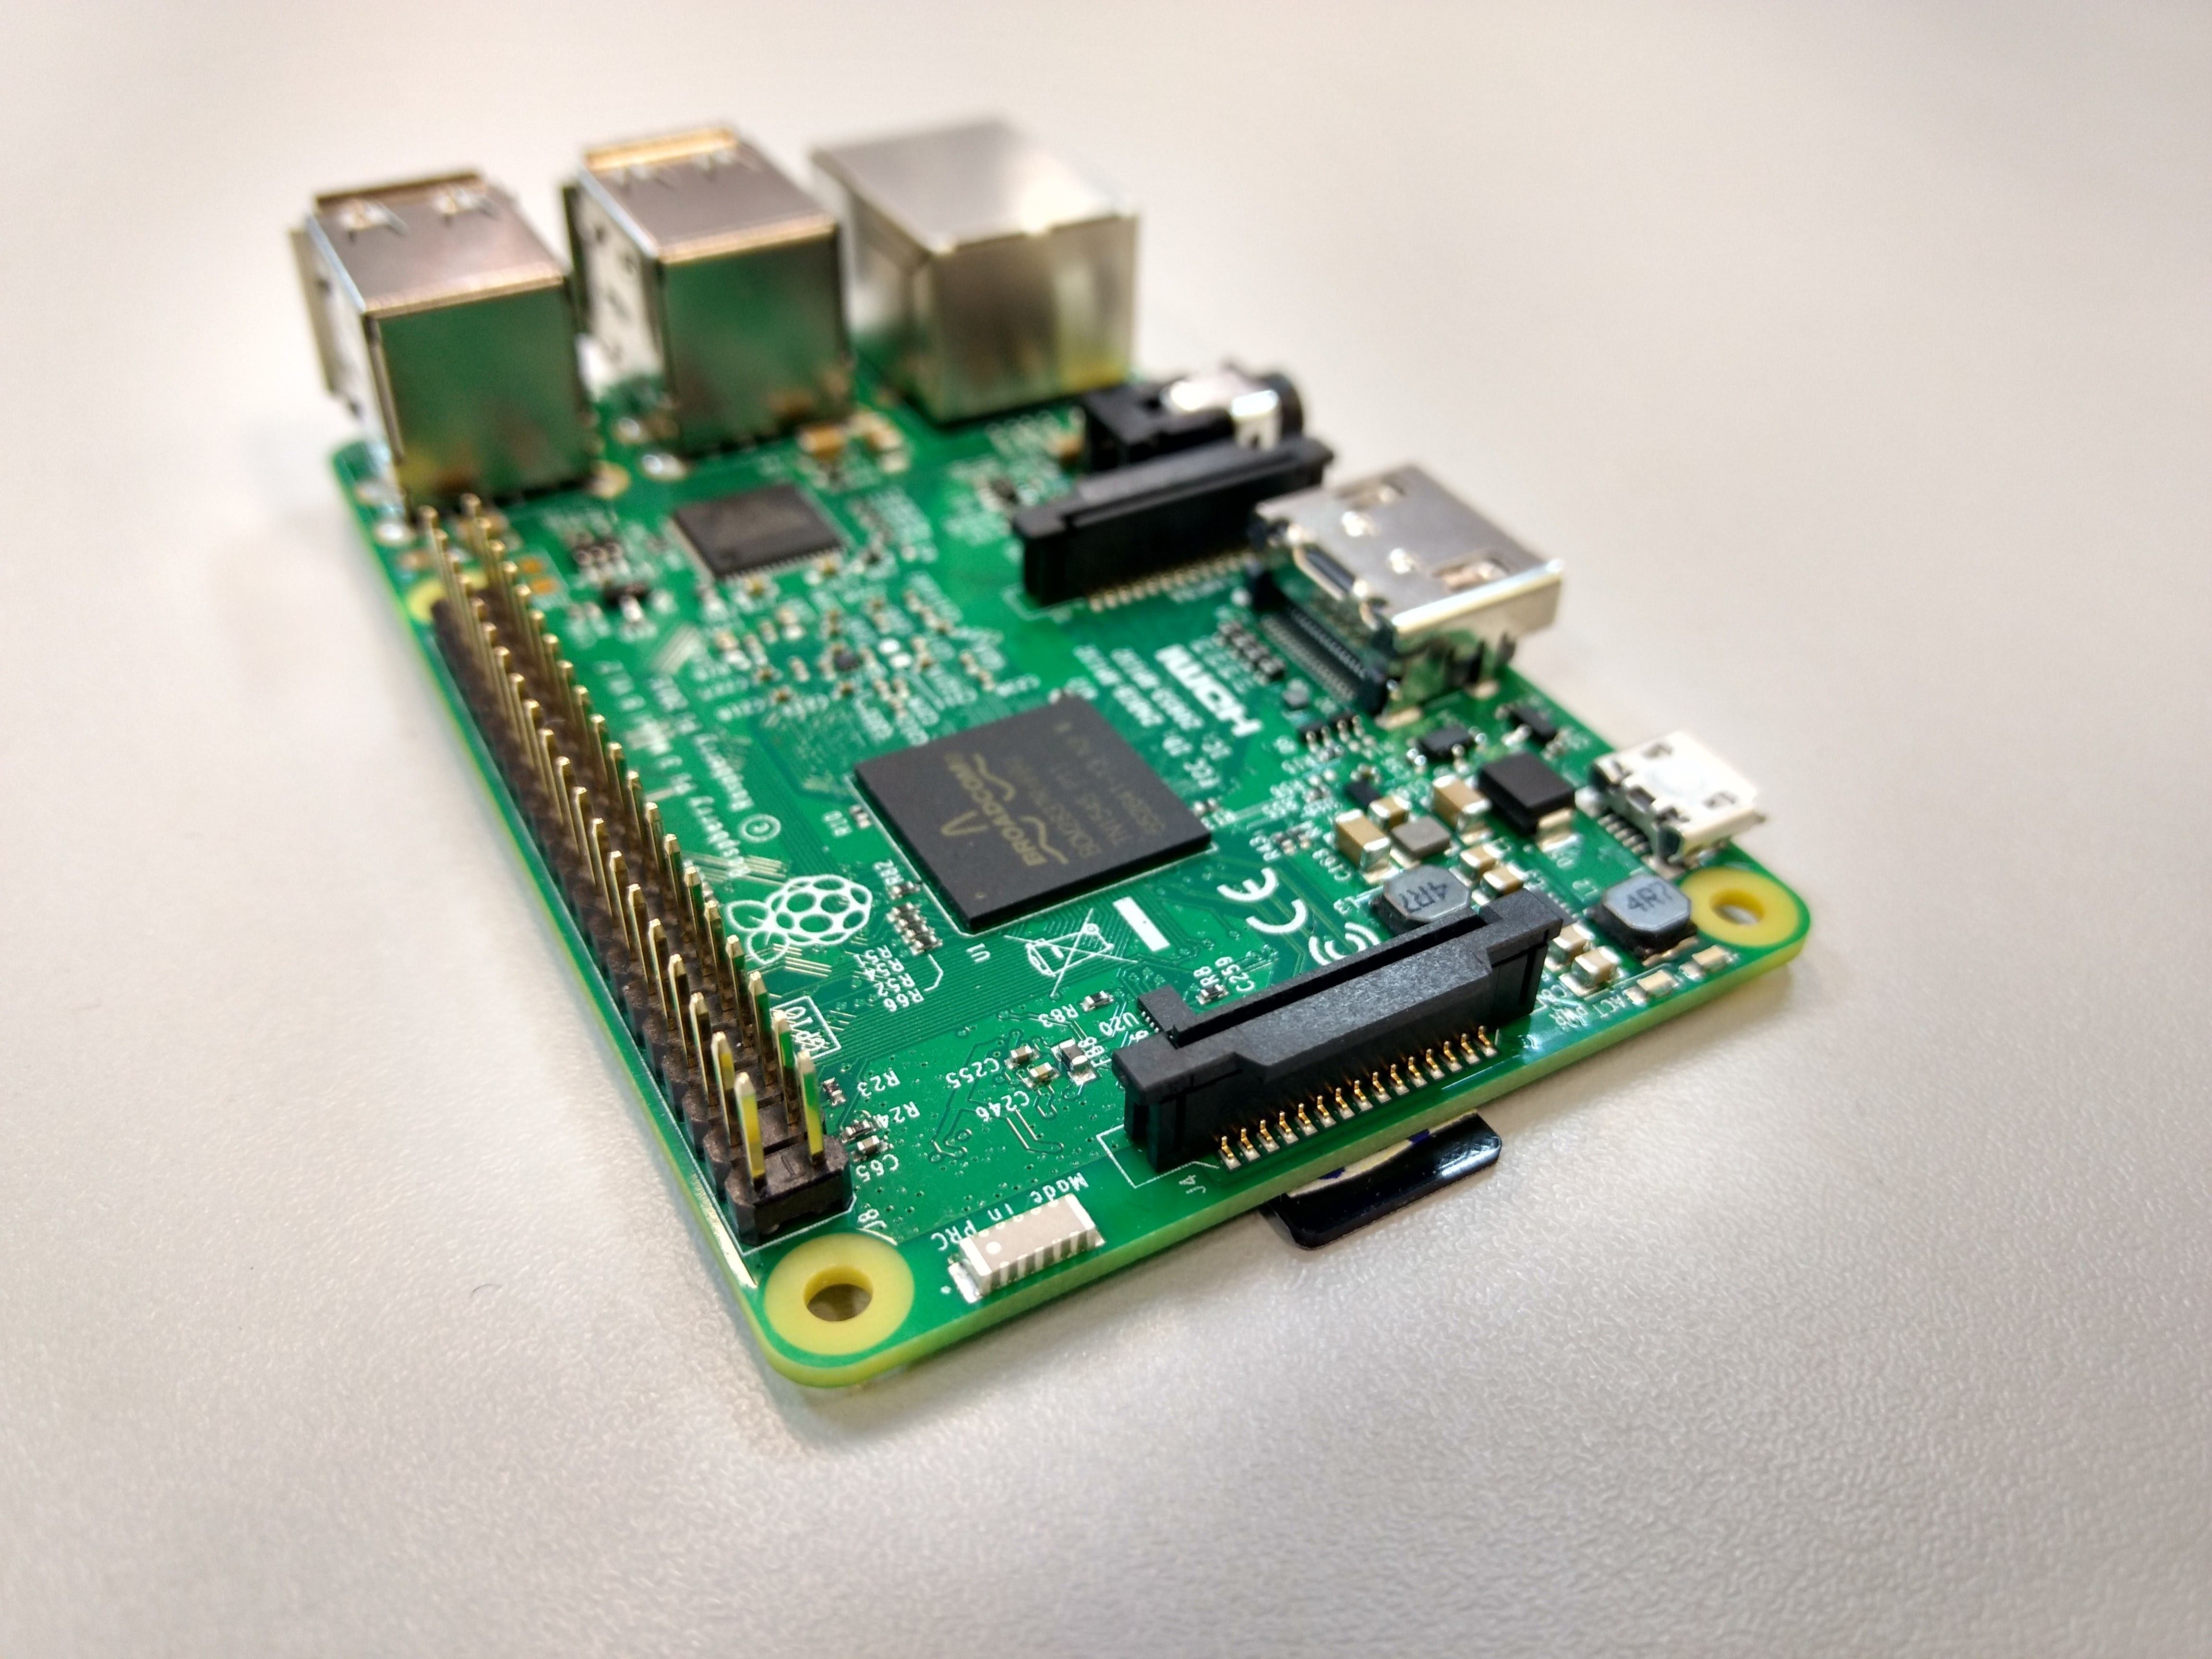
\includegraphics[width=1\textwidth]{040-plataformas/RPi-WiFi-dongles/rpi-onboard.jpg}
	\end{center}
	\legend{Fonte: Elaborada pelo autor}
\end{figure}



\subsection{Disponibilidade no mercado}
\label{subsec:mercado-rpi}

Para abordar a disponibilidade no mercado deve-se também contar os periféricos
que são necessários para desenvolver na plataforma RPI3 da mesma maneira que
foi feito com o ESP8266.

O RPI3 é ligado por uma fonte de 2A, 5V e 10W através de uma entrada micro
USB. Para ligá-lo, foi adquirido uma fonte USB tipo A para iPad, pois além de
poder desconectar o cabo da fonte, facilitando a manutenção, fornece a
quantidade exata de corrente que o computador precisa. A primeira aquisição foi
de um carregador de \emph{smartphone} que não forneceu os amperes necessários.

Em comparação com a plataforma anterior, esta tem uma exigência energética maior,
muito disto é devido a Wi-Fi integrado que é um destaque.
A antena de cerâmica do adaptador integrado pode ser vista no primeiro plano da
\autoref{fig-rpi-3}. Contudo, o adaptador não possui modo promíscuo e fez-se
necessário o uso de adaptadores Wi-Fi USB. As recomendações da comunidade
quanto a escolha do adaptador USB (também conhecido como \emph{dongle Wi-Fi})
são o Edimax EW-7811Un que não é tão comum no Brasil e o
EDUP EP-N85xx que tem muitos genéricos no mercado nacional.

Como camada de software, o RPI3 comporta diversos sistemas operacionais que são carregados de seu
cartão microSD. Alguns exemplos de sistemas compatíveis são
Archlinux, OpenELECE, Raspbian, Risc OS,
Pidora, Kali Linux, Windows 10 IoT, entre outros. Para este
trabalho, foi utilizado o Raspbian Jessie.

Portanto, para funcionamento e desenvolvimento de aplicações com RPI3 são
necessários componentes extra que são  demonstrados na
\autoref{table:custo-rpi}.

\begin{table}[htb]
\IBGEtab{%
\ABNTEXchapterfont {
	\caption{\label{table:custo-rpi}Descrição e custos com Raspberry Pi 3}%
}
}{%
\begin{tabular}{ccc}
\toprule
Produto								&	Descrição e utilização					&	Custo		\\
\midrule \midrule
Novo Raspberry Pi 3 (pi3)			&											&			 	\\
Quadcore 1.2ghz (10x+rapido) 1gb	&	Computador hospedeiro do sensor			&	R\$ 269,99	\\
\midrule
Fonte Carregador Original Usb		&	Fonte com conector USB tipo A que		&				\\
Apple Iphone 3 4 4s Ipad 1 2		&	supriu o consumo elétrico do RPI3		&	R\$ 13,99	\\
\midrule
Cabo USB com conectores 			&											&				\\
\emph{A} e \emph{Micro-B} 			&	Para conectar a fonte ao RPI3			&	R\$ 2,00^{1}	\\
\midrule
Cartão Micro Sdhc 16gb Ultra Sd 	&	Armazena o SO e outros arquivos, a		&				\\
Sandisk Classe 10 30mb/s			&	classe indica a velocidade do cartão	&				\\
									&	que implica na velocidade do SO			&	R\$ 21,99	\\
\midrule
Mini Adaptador Wireless Wifi 		&	Adaptador externo Wi-Fi que  			&				\\
Edup Usb 150mbps Raspberry Pi		&	permite modo promíscuo					&	R\$ 16,88	\\
\midrule
\bottomrule
\end{tabular}%
}{%
	\fonte{Produzido pelo autor.}%
	\nota[Nota 1]{Os cabos USB foram reutilizados de outras aplicações.}%
}
\end{table}


\subsection{Desenvolvimento e implantação}
\label{subsec:devel-rpi}

Para desenvolver com o RPI3 é necessário instalar um sistema operacional
em seu cartão SD, esse processo é simplificado com o uso do \emph{bootloader noobs}
que pode ser encontrado no site oficial do Raspberry para download \footnote{\url{https://www.raspberrypi.org/downloads/noobs/}}. Após
feito o download, os arquivos são extraídos do arquivo comprimido e colocados na
pasta raiz do cartão SD. Os próximos passos são conectar o cartão SD, a fonte,
monitor, teclado e mouse no RPi e ligar a fonte na tomada
para que imediatamente o computador ligue. Na tela inicial deve-se escolher uma rede com ou sem fio.
Após conectado, é possível escolher o sistema operacional que será baixado e instalado no próprio cartão SD.

O sistema operacional escolhido para a construção da plataforma de sensor foi o
Raspbian Jessie que é a distribuição Linux recomendada para o RPI. Nela, já estão
instaladas e configuradas muitas ferramentas utilizadas para o desenvolvimento e
	a implementação de projetos, como git, SSH e Node.js que foram utilizados para a
construção da aplicação como será discutido no próximo capítulo.

Para tornar o sistema completamente funcional para o desenvolvimento, é
necessário somente executar os passos de segurança e dar acesso remoto
ao sistema. Na interface gráfica de configuração do Raspbian, deve ser alterado
a senha do usuário ``pi'' e ativado o serviço SSH que permite acesso remoto através
de um terminal. Os últimos três passos são a atualização da lista de pacotes,
a atualização dos pacotes instalados e uma reinicialização do sistema para
garantir o bom funcionamento e segurança do mesmo.

Feito isto, qualquer desenvolvimento e implantação pode ser realizado com riscos
e falhas minimizados. Este processo é fundamental para a segurança da aplicação,
usuários e construtores, pois, como foi revelado após os ataques de 21 de Outubro
de 2016, dispositivos IoT atualmente não oferecem estes níveis mínimos de
segurança (software atualizado e senhas seguras), tornando-se um terreno
fértil para a construção de \emph{botnets} como foi o caso do \emph{malware
Mirai} utilizado para infectar milhões de dispositivos e causar o maior ataque
\emph{DDoS} até o momento com 1,2 terabits por segundo
\cite{guardianMirai} \cite{nytimesMirai}.


\subsection{Testes e resultados - Raspberry Pi}
\label{subsec:testes-rpi}

De maneira análoga à feita com o ESP8266, analisou-se a capacidade do Raspberry Pi
de operar com sua Wi-Fi em modo promíscuo, porém, devido a diferença de camada
de software envolvida, diferentes ferramentas foram utilizadas.

Neste caso, utilizou-se as ferramentas \emph{airodump-ng} \footnote{\url{https://www.aircrack-ng.org/doku.php?id=pt-br:airodump-ng}}
e TShark além das ferramentas de
Wi-Fi padrões do sistema operacional Raspbian. Para verificar o modo
promíscuo no ambiente Raspbian, utiliza-se os comandos ``ifconfig'',
``iwconfig'' e ``iw'', que são padrão do sistema operacional Debian, como
demonstrado a seguir.

\begin{lstlisting}[language=bash,caption={Ativação do modo monitor},label=code-iw-monitor]
pi@sensor-01:~ $ sudo ifconfig wlan0 down
pi@sensor-01:~ $ sudo iwconfig wlan0 mode monitor
pi@sensor-01:~ $ sudo ifconfig wlan0 up
\end{lstlisting}

O resultado pode ser observado com o comando a seguir.

\begin{lstlisting}[language=bash,caption={``iwconfig'' com modo monitor},label=code-check-monitor]
pi@sensor-01:~ $ sudo iwconfig wlan0
wlan0  IEEE 802.11bgn Mode:Monitor Frequency:2.412 GHz Tx-Power=20 dBm
	   Retry short limit:7   RTS thr:off   Fragment thr:off
       Power Management:off
\end{lstlisting}

Quando este processo foi realizado utilizando somente o adaptador de Wi-Fi
integrado no RPI3, cuja antena de cerâmica está em destaque na
\autoref{fig-rpi-onboard}, o resultado foi negativo, portanto outros adaptadores
foram necessários.

No ambiente do laboratório (LTIA),
encontrou-se adaptadores Wi-Fi USB D-link
(\autoref{fig-dlink}), porém executando o mesmo teste neles não foi possível
ativar o modo promíscuo. Um terceiro adaptador emprestado foi o modelo Ralink Edup A (\autoref{fig-ralink-edup}) que teve resultado
positivo. Para a construção dos dois sensores foi necessária a aquisição e
subsequente teste de mais um modelo de adaptador, Ralink Edup B (\autoref{fig-ralink}), que está listado na
\autoref{table:custo-rpi}, porém a sua
aparência externa difere do anterior, mesmo que a aquisição foi do mesmo anúncio.

\begin{figure}[htb]
 \label{adaptadores-usb}
 \centering
  \begin{minipage}{0.49\textwidth}
    \centering
    \caption{Antena cerâmica de Wi-Fi e Bluetooth do Raspberry Pi 3 \label{fig-rpi-onboard}}
    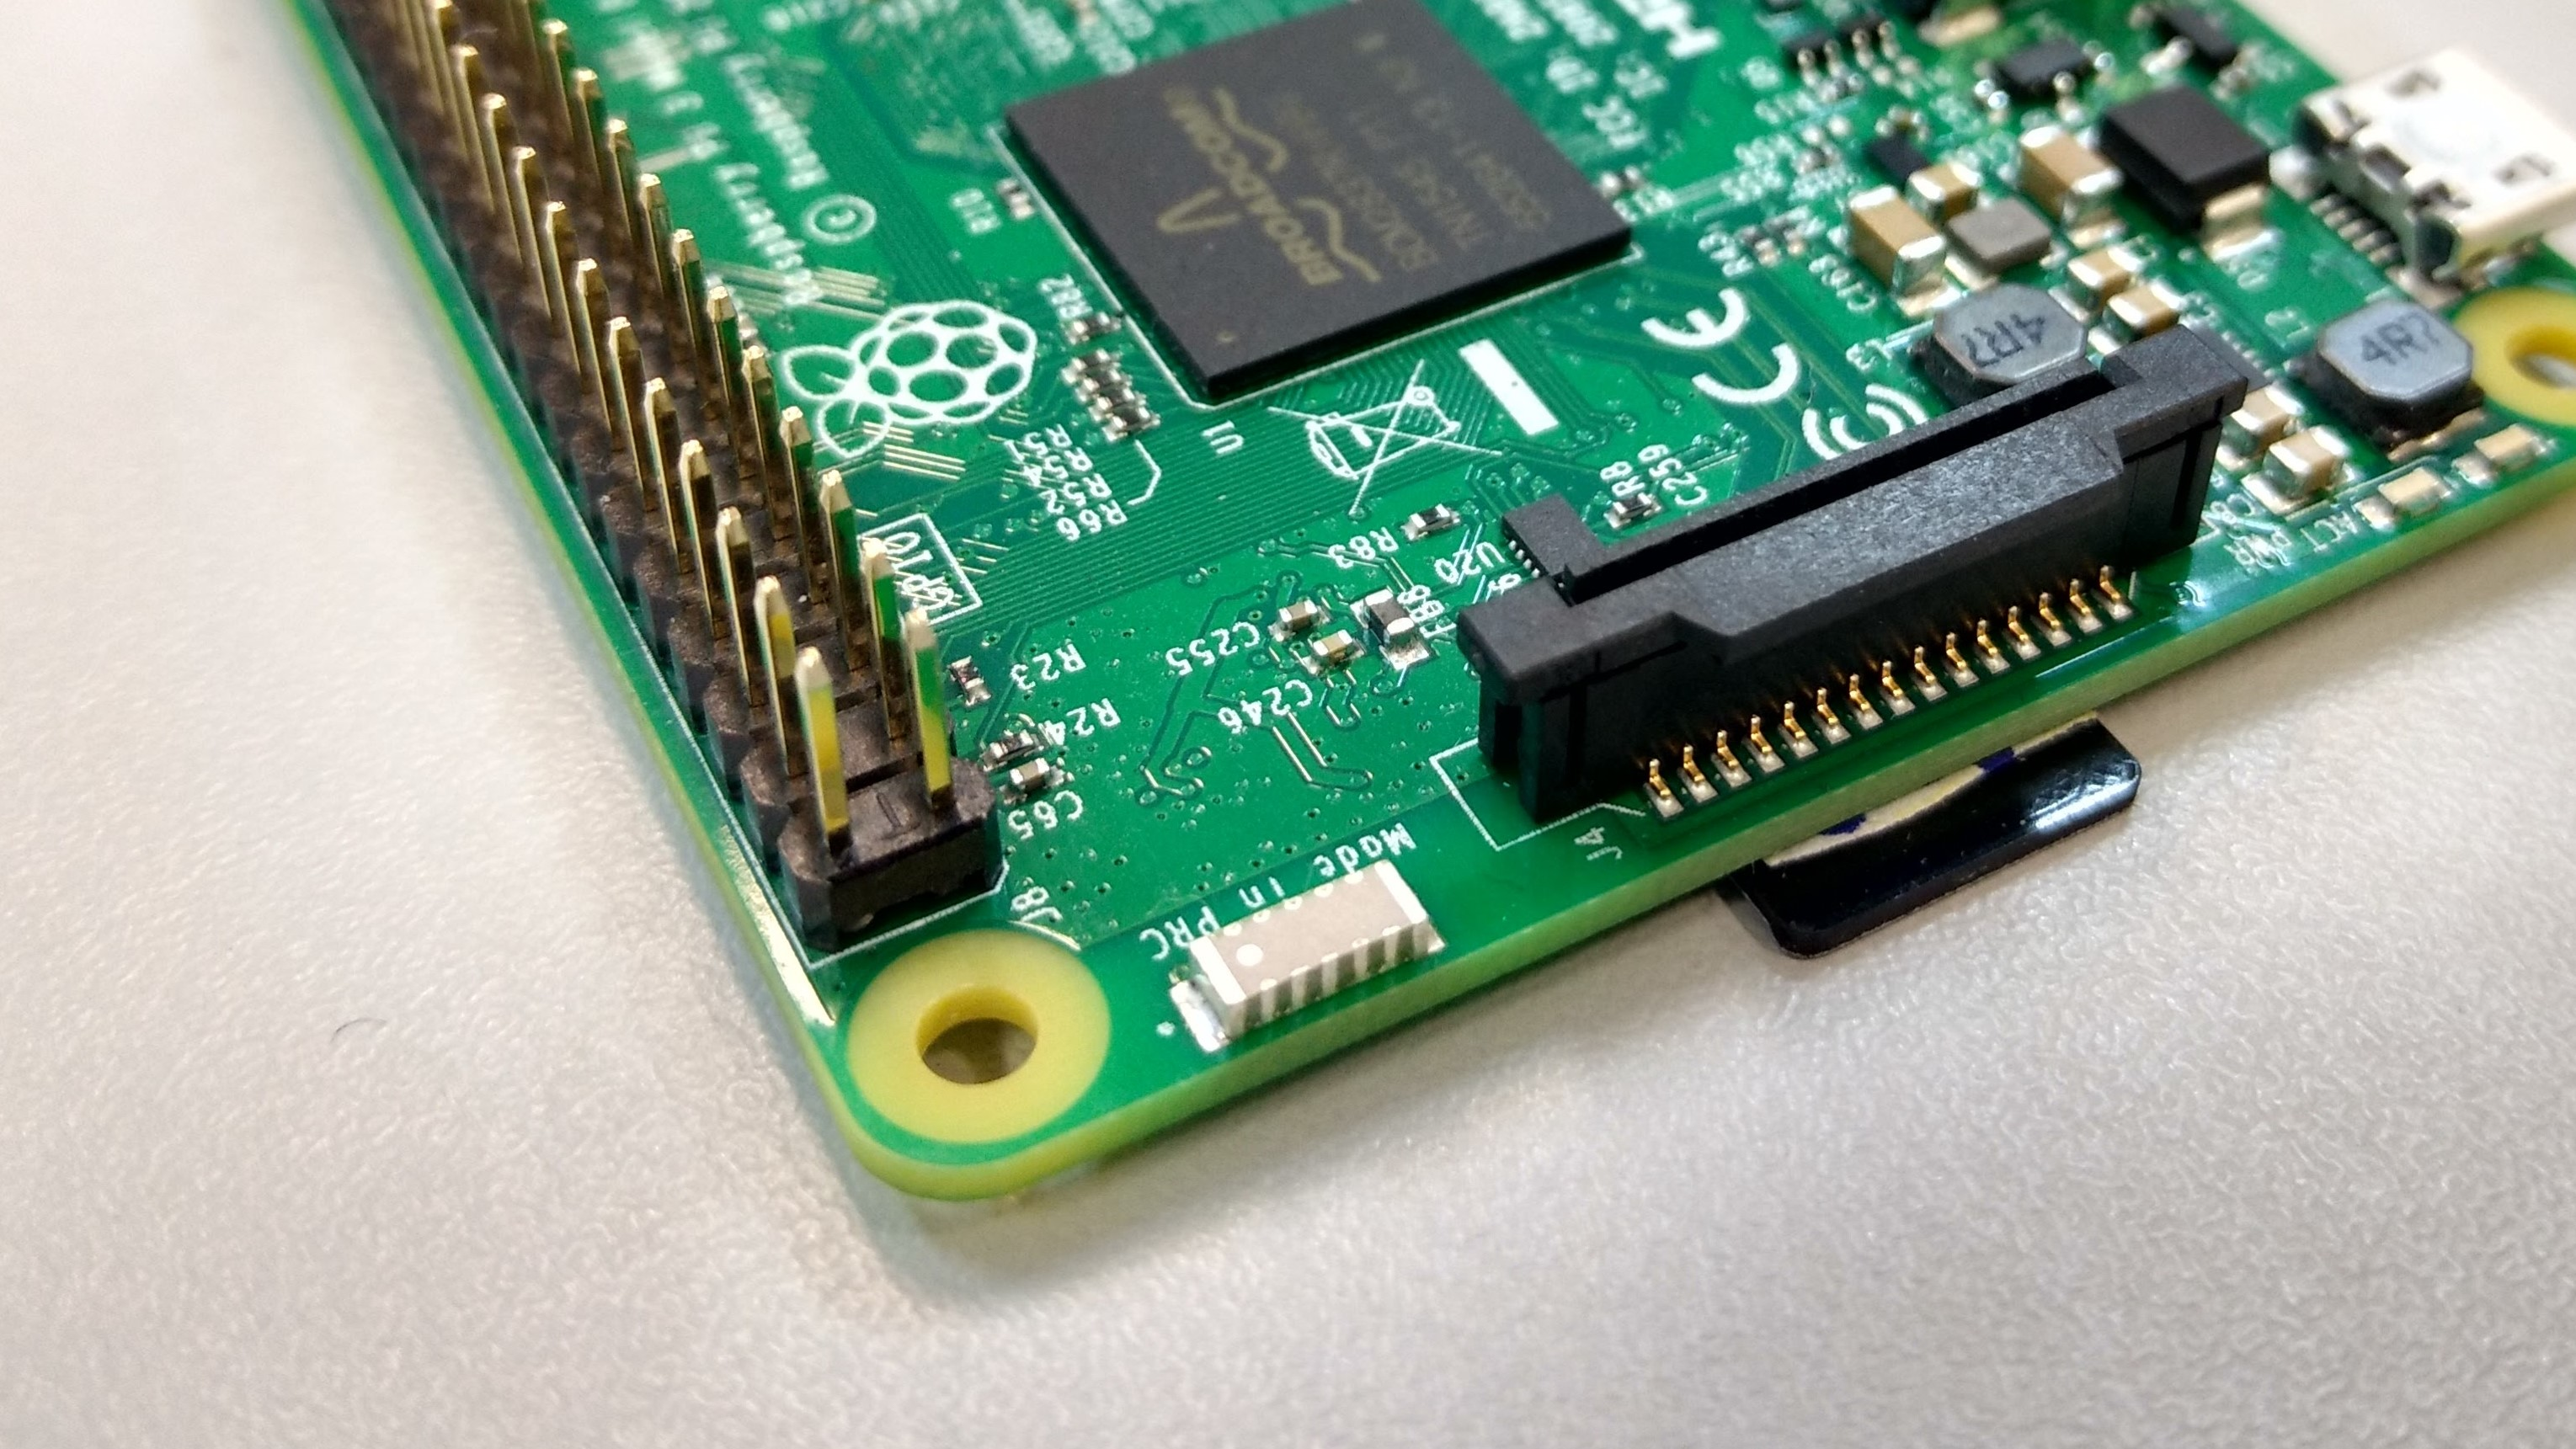
\includegraphics[width=1\textwidth]{040-plataformas/RPi-WiFi-dongles/cut_rpi-onboard.jpg}
    \legend{Fonte: Produzido pelo autor}
  \end{minipage}
  \hfill
  \begin{minipage}{0.49\textwidth}
	\centering
  	\caption{Adaptador Wi-Fi USB D-Link do laboratório \label{fig-dlink}}
  	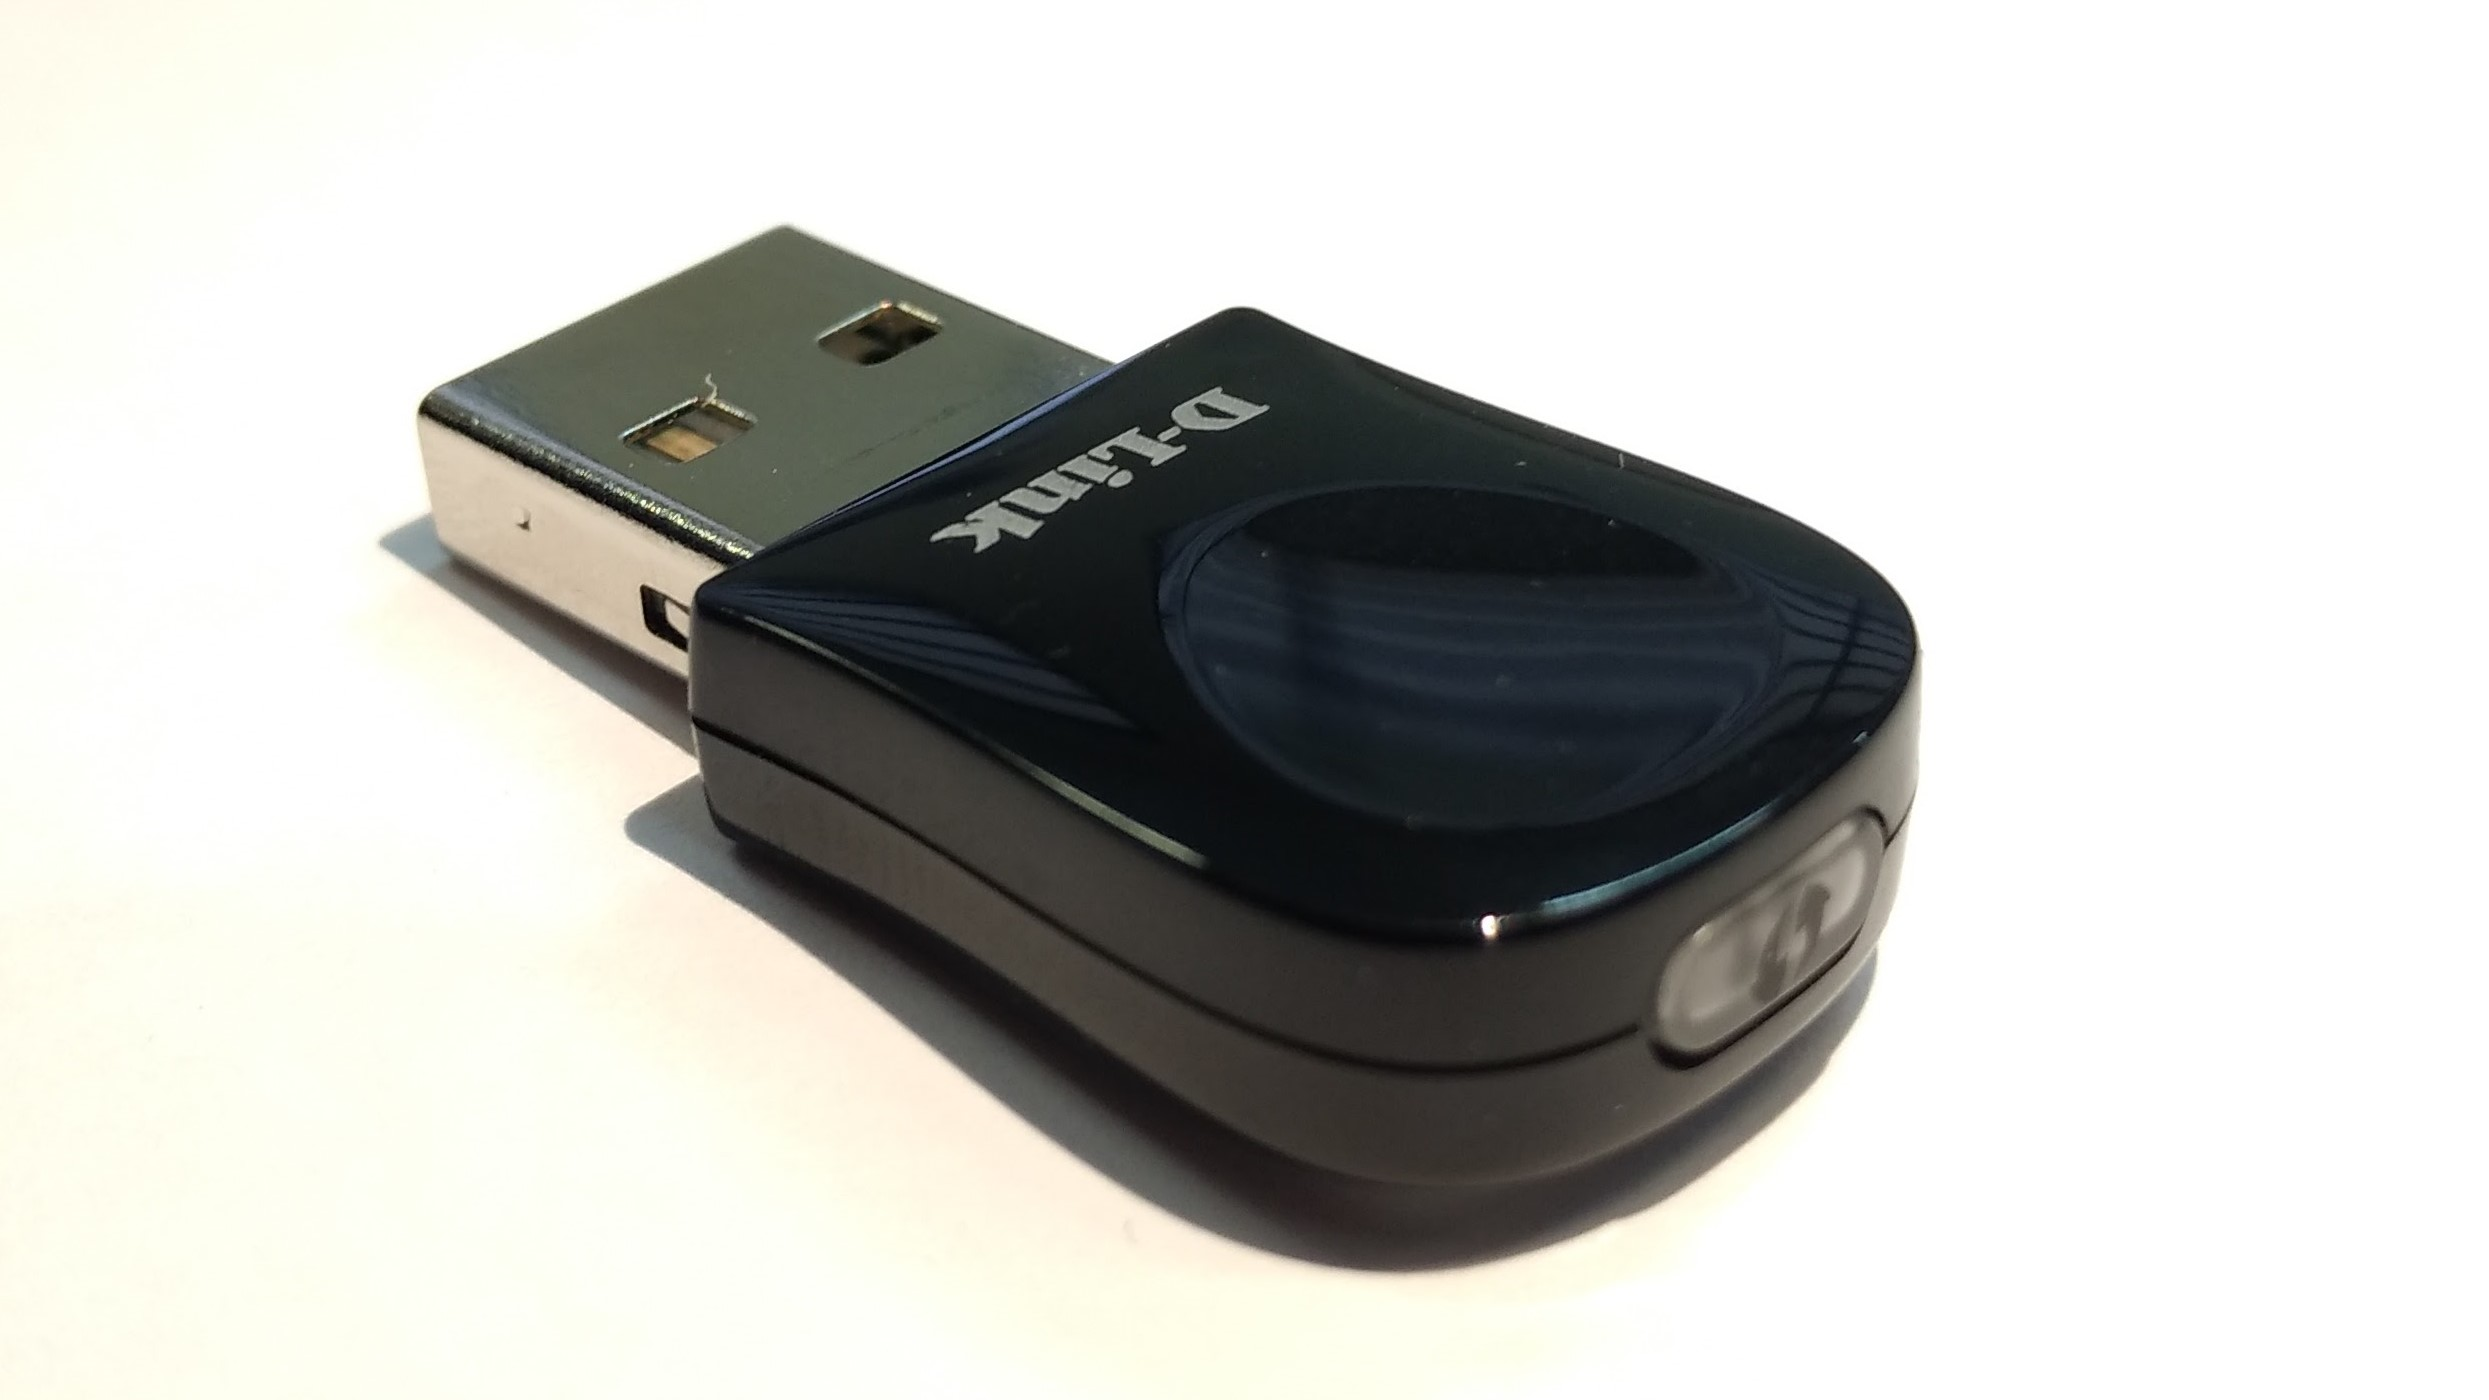
\includegraphics[width=1\textwidth]{040-plataformas/RPi-WiFi-dongles/cut_dlink.jpg}
  	\legend{Fonte: Produzido pelo autor}
  \end{minipage}
\end{figure}

\begin{figure}[htb]
 \label{adaptadores-usb-2}
  \begin{minipage}{0.45\textwidth}
	  \centering
	  \caption{Adaptador Wi-Fi USB Ralink Edup A\label{fig-ralink-edup}}
	  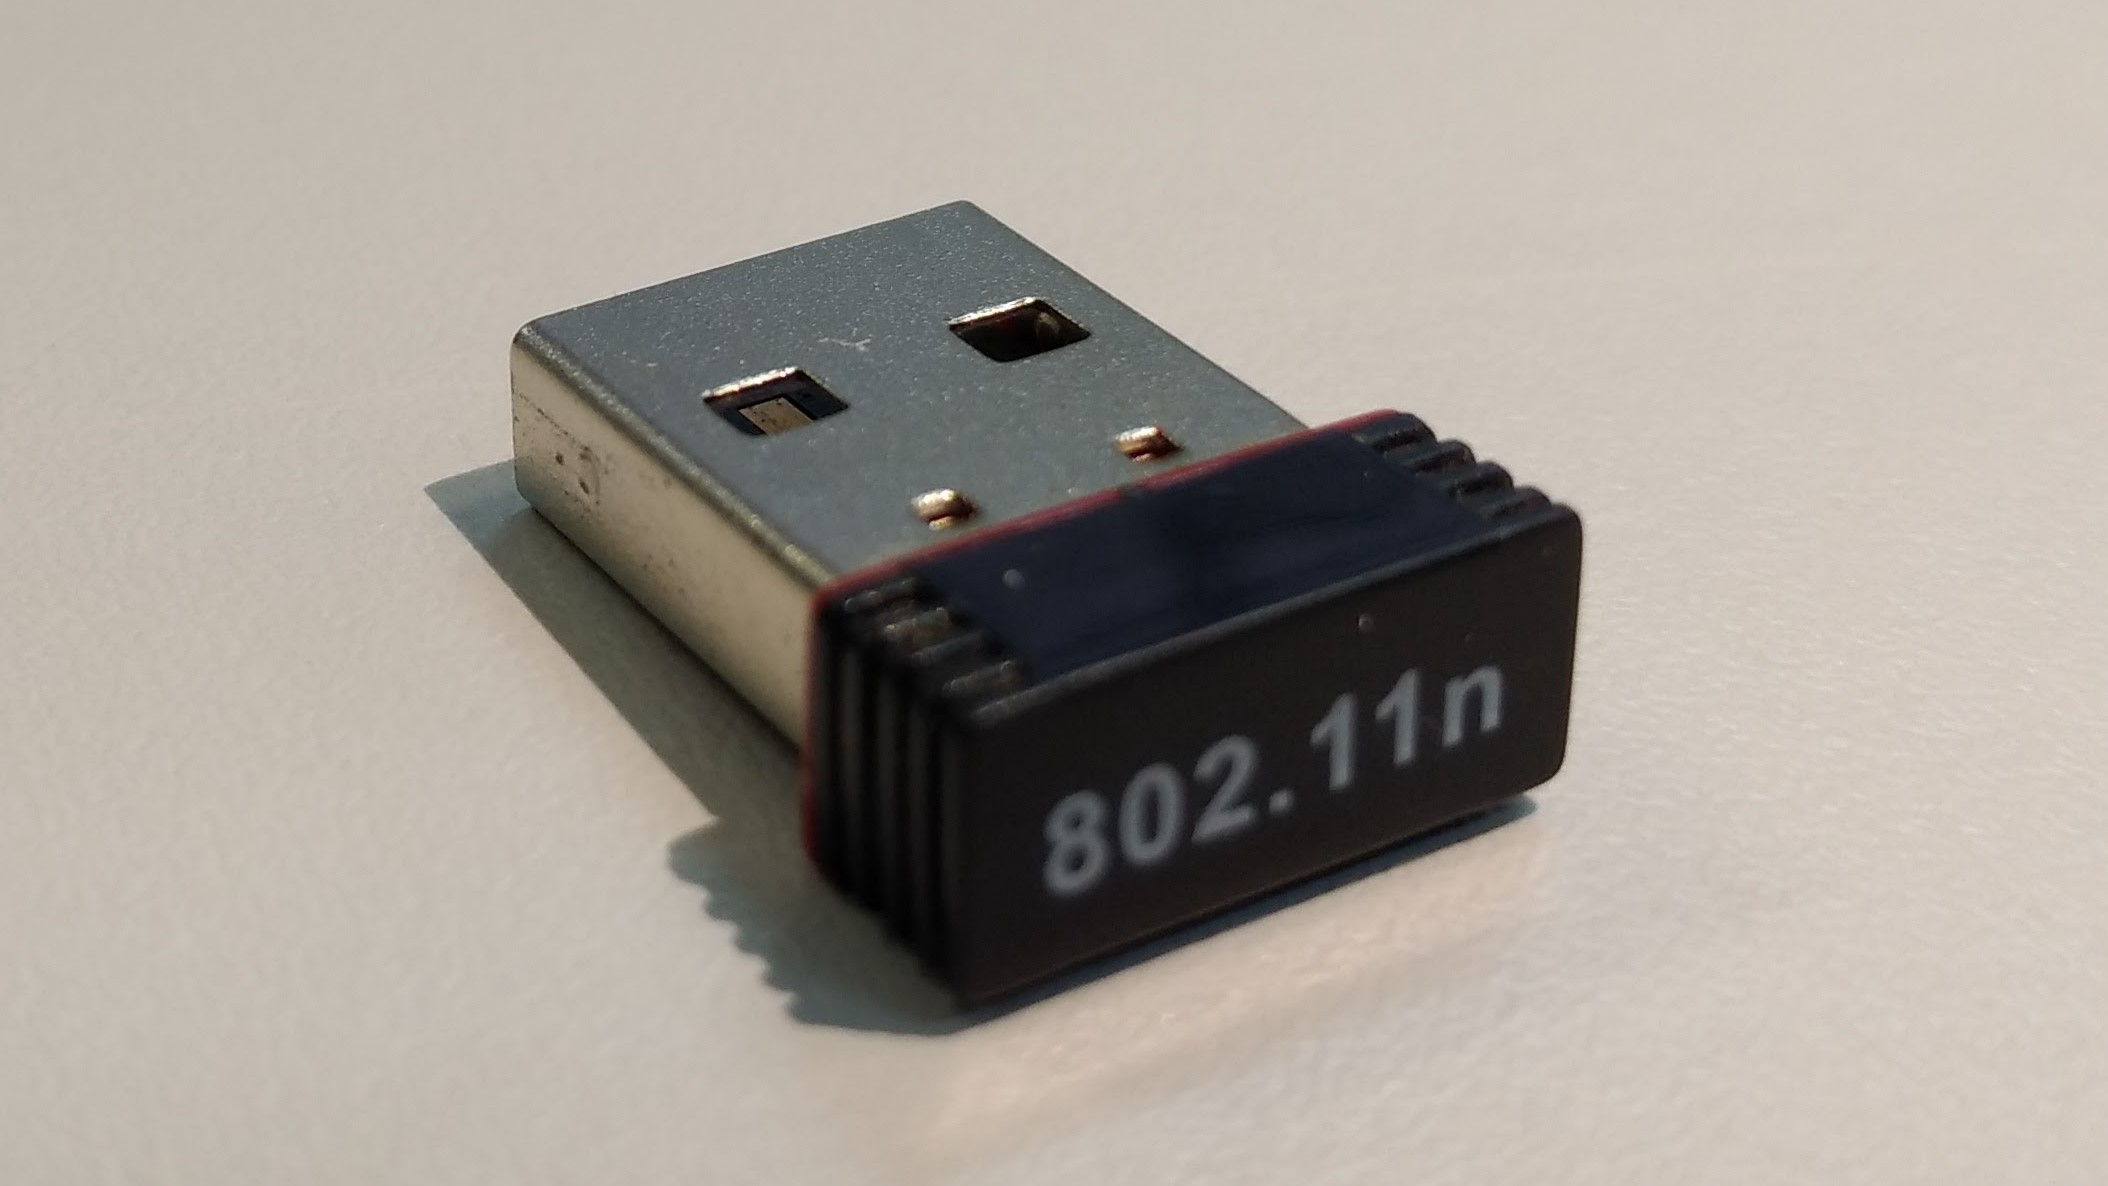
\includegraphics[width=1\textwidth]{040-plataformas/RPi-WiFi-dongles/cut_ralink-epub.jpg}
	  \legend{Fonte: Produzido pelo autor}
  \end{minipage}
  \hfill
  \begin{minipage}{0.45\textwidth}
	  \centering
	  \caption{Adaptador Wi-Fi USB Ralink Edup B\label{fig-ralink}}
	  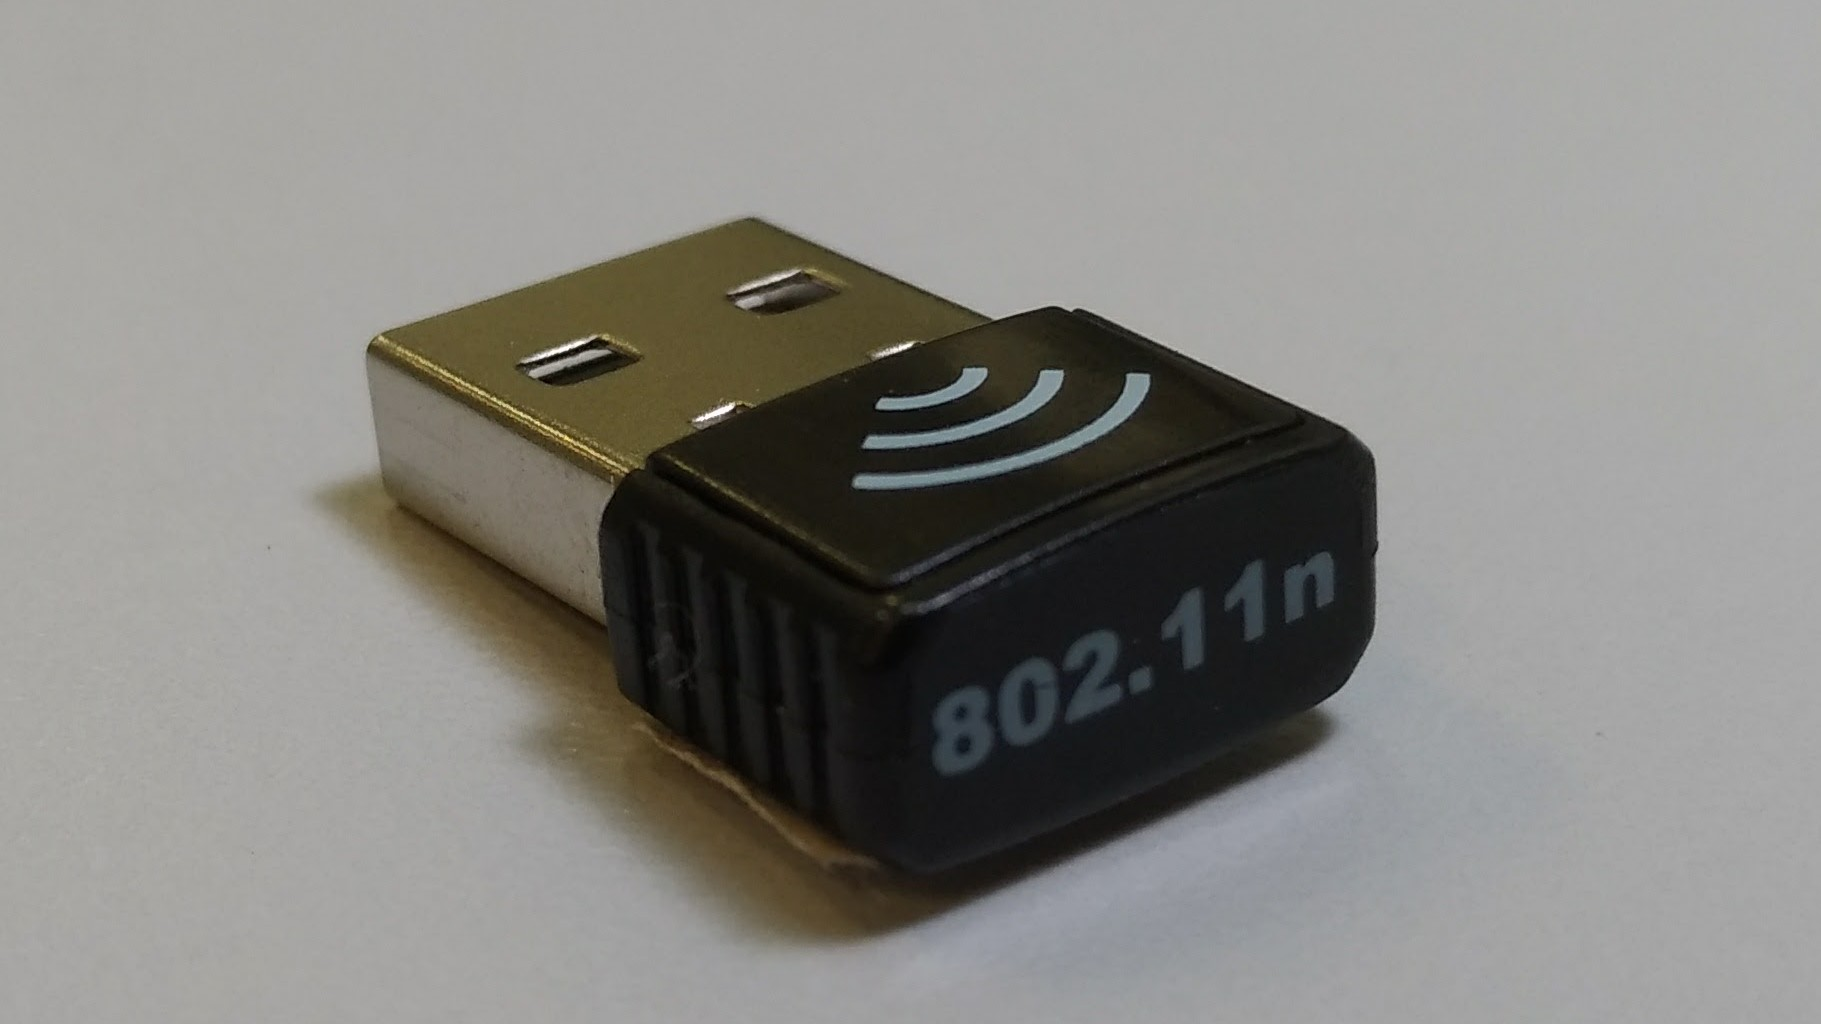
\includegraphics[width=1\textwidth]{040-plataformas/RPi-WiFi-dongles/cut_ralink.jpg}
	  \legend{Fonte: Produzido pelo autor}
  \end{minipage}
\end{figure}


Para capturar e avaliar pacotes uma ferramenta é necessária. Na área
de segurança da informação pode-se encontrar o airodump-ng que é utilizado para
avaliar e explorar vulnerabilidades de segurança em redes Wi-Fi. Outra área que
forneceu uma ferramenta adequada foi a área de qualidade de serviço em redes de
computadores (QoS) onde o software Wireshark é bem popular, uma interface alternativa
do mesmo feita para uso em terminal é chamada TShark.

Para testar a viabilidade do sensor, utilizou-se o \emph{airodump-ng} que é uma
ferramenta de terminal interativa, como vista na \autoref{fig-airodump}, onde é
demonstrado a capacidade de capturar pacotes do tipo \emph{Beacon} (tabela com
``BSSID'', ``PWR'' e ``Beacons'' na parte superior da \autoref{fig-airodump}) que anunciam
a presença de AP e o nome da rede que
ele está servindo. Além disso, é possível observar também os pacotes entre os dispositivos ``Stations''
associados a um AP (tabela com ``BSSID'', ``STATION'' e ``PWR'' na parte inferior da
\autoref{fig-airodump}). Em ambos os casos, é mostrado um valor de RSS
(``PWR'') associado a cada transmissor, portanto, demostrando a viabilidade
do sensor com a informação de potência de sinal.

\begin{figure}[htb]
	\caption{\label{fig-airodump}Interface do airodump-ng}
	\begin{center}
	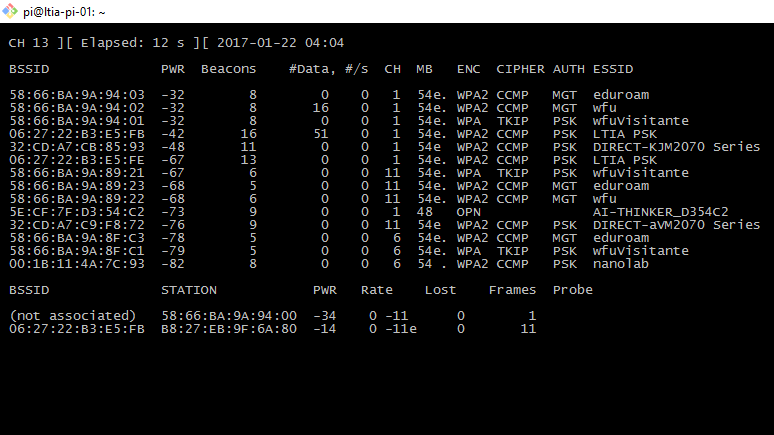
\includegraphics[width=1\textwidth]{040-plataformas/RPi-WiFi-dongles/wifi-sniff-rpi/4-rpi-airodump.png}
	\end{center}
	\legend{Fonte: Elaborada pelo autor}
\end{figure}


Após a avaliação de viabilidade, fez-se necessário o uso de uma aplicação mais
flexível do que o airodump-ng onde fosse possível escolher campos e gerar
relatórios mais flexíveis. Para essa tarefa o software TShark mostrou-se
ideal.

Nele, pode-se escolher, através de argumentos na execução por terminal, a
interface com a opção “-i wlan0”, o modo monitor com opção “-I”, a opção “-T
fields” que altera o funcionamento normal dele para que com as opções “-e
field.field\_child” seja permitido escolher os campos mostrados e juntamente com
as opções “-E separator=, -E quote=d” o formato do relatório gerado torna-se CSV
(\emph{comma separated values} - valores separados por vírgula).

Desta maneira, todos os pacotes capturados são processados pelo TShark e
escritos na saída padrão do terminal (\emph{stdout}), dando a possibilidade de
usar a ferramenta de criação de arquivo, acrescentar em arquivo e redirecionar
para outro processo do terminal Linux (respectivamnte ‘>’, ‘»’ e ‘|’). Esta
capacidade, ausente no airodump-ng, é essencial para este trabalho.

Para este trabalho, o comando mais utilizado foi o que mostra os endereços MAC
de origem e transmissão (``wlan.sa'', ``wlan.ta''), os mesmos endereços, porém com nome
de fabricante como prefixo (``wlan.sa\_resolved'', ``wlan.ta\_resolved''), a potência de
sinal (``radiotap.dbm\_antsignal'') e o nome da rede anunciada se o pacote for um
\emph{Beacon}, da mesma maneira que o airodump-ng mostra.

\begin{lstlisting}[language=bash,caption={TShark e opções},label=code-tshark]
pi@sensor-01:~ $ tshark -I -i wlan0 -T fields -E header=y -E quote=d \
-e wlan.sa -e wlan.sa_resolved -e wlan.ta -e wlan.ta_resolved \
-e radiotap.dbm_antsignal -e wlan_mgt.ssid
\end{lstlisting}

Por último, a configuração padrão do TShark não recomenda a execução em modo
supervisor (``root'') por motivo de segurança. Para executá-lo, o usuário precisa ser do
grupo ``wireshark''. Para adicionar o usuário ``pi'' ao grupo ``wireshark'', utiliza-se o comando do
\autoref{code-usermod}.

\begin{lstlisting}[language=bash,caption={Adição do usuário pi ao grupo wireshark},label=code-usermod]
pi@sensor-01:~ $ sudo usermod -a -G wireshark pi
\end{lstlisting}

Este modo de operação permite executar a aplicação final sem necessidade de
elevação de privilégios (\emph{root}), tornando-a mais segura, pois mesmo que
aplicação seja subvertida o sistema operacional não poderá ser comprometido.

\section{Escolha e conclusão}
\label{sec:escolha-plataforma}

Em comparação com o ESP8266, o RPI3 compensou seu custo elevado devido a
facilidade de programação, acesso aos seus recursos e acesso a recursos externos uma
vez que foi possível chegar ao modo promíscuo facilmente através de recursos nativos do
sistema operacional. Para uma comparação das plataformas veja a \autoref{table:comp-hardware-esp-rpi}.

\begin{table}[htb]
\IBGEtab{%
\ABNTEXchapterfont {
	\caption{Comparação das plataformas ESP8266 e RPI3}%
	\label{table:comp-hardware-esp-rpi}
}
}{%
\begin{tabular}{cccc}
\toprule
Aspecto				&	 Raspberry Pi 3 model B					&	ESP-12f		\\
\midrule \midrule
GPIO				&	 27 GPIOs (0 a 26) digitais				&	17 GPIOs digitias e analógicos		\\
\midrule
Número de pinos		&	 40 pinos								&	22 pinos	\\
\midrule
Processamento		&	\emph{ARMv8 64-bit quad-core 1.2 GHz}	&	\emph{Tensilica L106 32-bit (MCU)} com 80		\\
					&	e \emph{VideoCore IV 3D GPU}			&	ou 160 MHz e instruções \emph{16-bit RSIC}	\\
\midrule
Memória RAM			&	  1 GB									&	RAM < 50 kB	\\
\midrule
Memória longo termo	&	 cartão SD (usualmente 8 ou 16 GB)		&	\emph{SPI flash} de 4 MB		\\
\midrule
Tamanho físico		&	 85x56mm								&	 24x13mm	\\
\midrule
Rede embutida		&	 Megabit Ethernet, 802.11 b/g/n			&	802.11 b/g/n	\\
\midrule
Expansão			&	  USB, DSI, CSI e GPIO					&	Somente GPIO	\\
\midrule
Sistema operacional	&	  Qualquer linux/windowns/risc			&	\\
					&	  compilado em ARMv8					&	Não possui	\\
\midrule
Custo				&	 de R\$ 190,00 a R\$ 270,00				&	 de R\$ 12,56 a R\$ 35,87		\\
\midrule
\bottomrule
\end{tabular}%
}{%
	\fonte{Produzido pelo autor.}%
}
\end{table}

O RPI3 foi adotado como plataforma para o sensor de detecção de dispositivos,
pois o modo promíscuo (\emph{monitor mode}) conseguiu ser acessado através de adaptador
USB Wi-Fi. Apesar do esforço para ativação do modo promíscuo na plataforma ESP8266, o uso desta reduziria
significativamente o custo de cada sensor. Para comparação do custo da aplicação
aqui proposta, veja a \autoref{table:comp-app-sensor}.

\begin{table}[ht]
\IBGEtab{%
\ABNTEXchapterfont {
	\caption{Comparação de custos para o sensor da aplicação proposta em função da plataforma}%
	\label{table:comp-app-sensor}
}
}{%
\begin{tabular}{c|cr|cr}
	\toprule
	\multicolumn{5}{c}{Sensor} \\
	\midrule
	Plataforma				&	\multicolumn{2}{|c|}{Raspberry Pi}		&	\multicolumn{2}{|c}{ESP8266}	\\
	\midrule
	Item					&	Descrição			&	Custo em R\$	&	Descrição					&	Custo em R\$	\\
	\midrule
	Plataforma				&	RPI3				&	269,99			&	D1 mini (ESP-12f)			&	12,56	\\
	Fonte de alimentação	&	Fonte Usb iPad		&	13,99			&	Fonte Usb Celular com cabo	&	7,85	\\
												&	Cabo Usb A-micro	&	2,00			&								&		\\
	Adaptador Wi-Fi 		&	Edup Usb			&	16,88			&								&		\\
	Memória			 		&	SD c10 16GB			&	21,99			&								&		\\
	\midrule
	Total por Sensor		&						&	324,85			&								&	20,41	\\
	\midrule\midrule
\end{tabular}%
}{%
	\fonte{Produzido pelo autor.}%
}
\end{table}

É importante notar a proporção de custo entre as duas plataformas onde o RPI3
custa aproximadamente 15 vezes mais por sensor do que a plataforma ESP8266. Isto
justifica o esforço realizado durante o desenvolvimento deste trabalho para
explorar e, com esperança, ativar o modo promíscuo no pequeno dispositivo que
infelizmente não rendeu frutos.

Para a construção do Gateway IoT, as exigências de hardware são
capacidades mínimas de processamento,
armazenamento e comunicação, e a exigência de software é um sistema
operacional que suporte um MQTT Broker. Portanto, para o \emph{gateway}, a
plataforma ESP8266 claramente não é adequada, então um RPI3 representa o custo mínimo.

\begin{table}[ht]
\IBGEtab{%
\ABNTEXchapterfont {
	\caption{Custos para o \emph{gateway} da aplicação proposta}%
	\label{table:custo-app-gw}
}
}{%
\begin{tabular}{c|cr}
	\toprule
	\multicolumn{3}{c}{Gateway}\\
	\midrule
	Item					&	Descrição			&	Custo em R\$	\\
	\midrule
	Plataforma				&	RPI3				&	269,99			\\
	Fonte de alimentação	&	Fonte Usb iPad		&	13,99			\\
												&	Cabo Usb A-micro	&	2,00			\\
	Memória			 		&	SD c10 16GB			&	21,99			\\
	\midrule
	Total por Gateway		&						&	307,97			\\
	\midrule
	\bottomrule
\end{tabular}%
}{%
	\fonte{Produzido pelo autor.}%
}
\end{table}
